\documentclass[11pt,a4paper,english]{article}
\usepackage{babel}
\usepackage[utf8]{inputenc}
\usepackage{amsmath}
\usepackage{amsfonts}
\usepackage{amssymb}
\usepackage{graphicx}
\usepackage{natbib}
\usepackage{bbm}
\usepackage{tabularx,booktabs}
\newcommand\numberthis{\stepcounter{equation}{}\tag{Equation \theequation}}
\newcolumntype{B}{>{\centering\arraybackslash}X}

\addtolength{\oddsidemargin}{-.895in}
	\addtolength{\evensidemargin}{-.895in}
	\addtolength{\textwidth}{1.75in}

\addtolength{\topmargin}{-1.25in}
	\addtolength{\textheight}{1.75in}

%\author{Joelle Mbatchou}
\title{Binary Trait Association testing using Retrospective approach with MCMCglmm}
%\date{\vspace{-6ex}Oct. $9^{\text{th}}$ 2015}
\date{\vspace{-7ex}}
\begin{document}
\maketitle

The sample constitutes of 45 3-generations families with 22 individuals in each family ($n=990$). Given the covariates, genotypes and random effects, we generate the binary phenotype according to the following logistic mixed model
\begin{align*}
Y_i|\pi_i &\sim \text{Ber}(\pi_i),\\
\text{logit}(\pi_i) &=  \;\beta_0 + \beta_1\, \text{age}_i + \beta_2\, \text{sex}_i + \beta_3\, \text{Z}_i \numberthis\\
&\;\;\; +\lambda \mathbbm{1}_{\{W_{1i}\,>\,0,W_{2i}\,>\,0\}} + U_i,\\
 \mathbf{U} &\sim \; MVN(0, \sigma_a^2\, \Phi),
\end{align*}
where we include the genotype vectors of two causal unobserved common variants $\mathbf{W}_1$ and $\mathbf{W}_2$ (MAF is 0.1 and 0.2 respectively) coded as 0,1 or 2 (i.e. the minor allele count) and $\lambda$ denotes their epistatic effect on the phenotype. We also include three covariates that affect the trait: age, sex and a $N(0,1)$ covariate $\mathbf{Z}$ and the intercept term $\beta_0$ is chosen so that the mean prevalence is 11\%. We include phenotype-based ascertainment where only families with at least 6 ($\sim 22\%$) affected individuals are included in the sample.

We generate 1000 trait replicates and perform association testing with the first of the two causal genes. To get power, we count the proportion of these p-values that are less than our significance level threshold of 0.05. Note that the upper bound for the SE for power will be 0.016. 

We consider different proportions for the amount of total variability explained by the Bernoulli error and also vary the proportion of the variability, on the logit scale, due to the additive polygenic effects relative to that due to the covariates.

\vspace{.4cm}
$\bullet$
The mean penetrance is about 21\% for individuals that have at least one mutation at both causal loci compared to 10\% for individuals that don't have any mutation at one (or both) of the two loci. 
\end{document}
\begin{center}
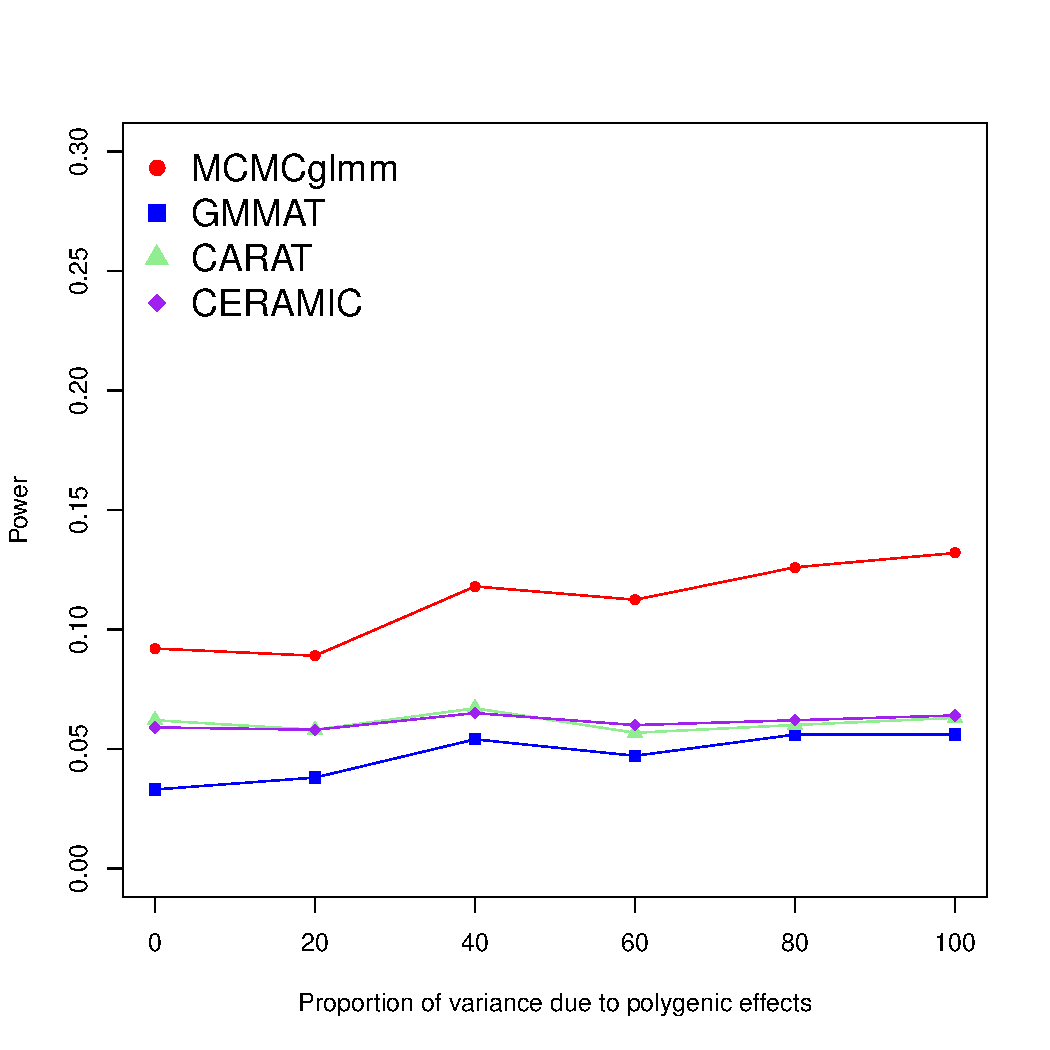
\includegraphics[scale=.45]{power_plot20.pdf}
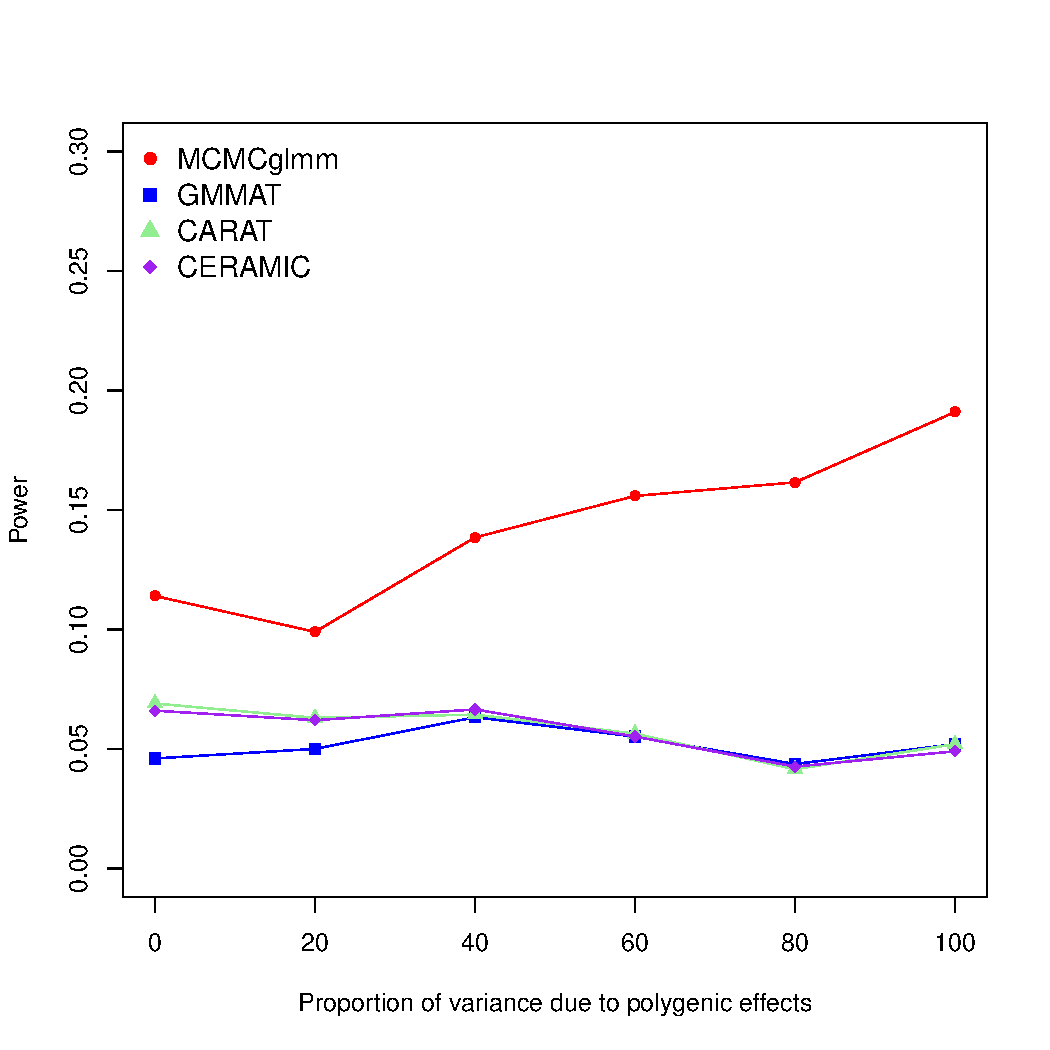
\includegraphics[scale=.45]{power_plot40.pdf}
\includegraphics[scale=.45]{power_plot60.pdf}
\end{center}
%\newpage
%$\bullet$
%The mean penetrance is about 15\% for individuals that have at least one mutation at both causal loci compared to 10\% for individuals that don't have any mutation at one (or both) of the two loci. 
%
%\begin{center}
%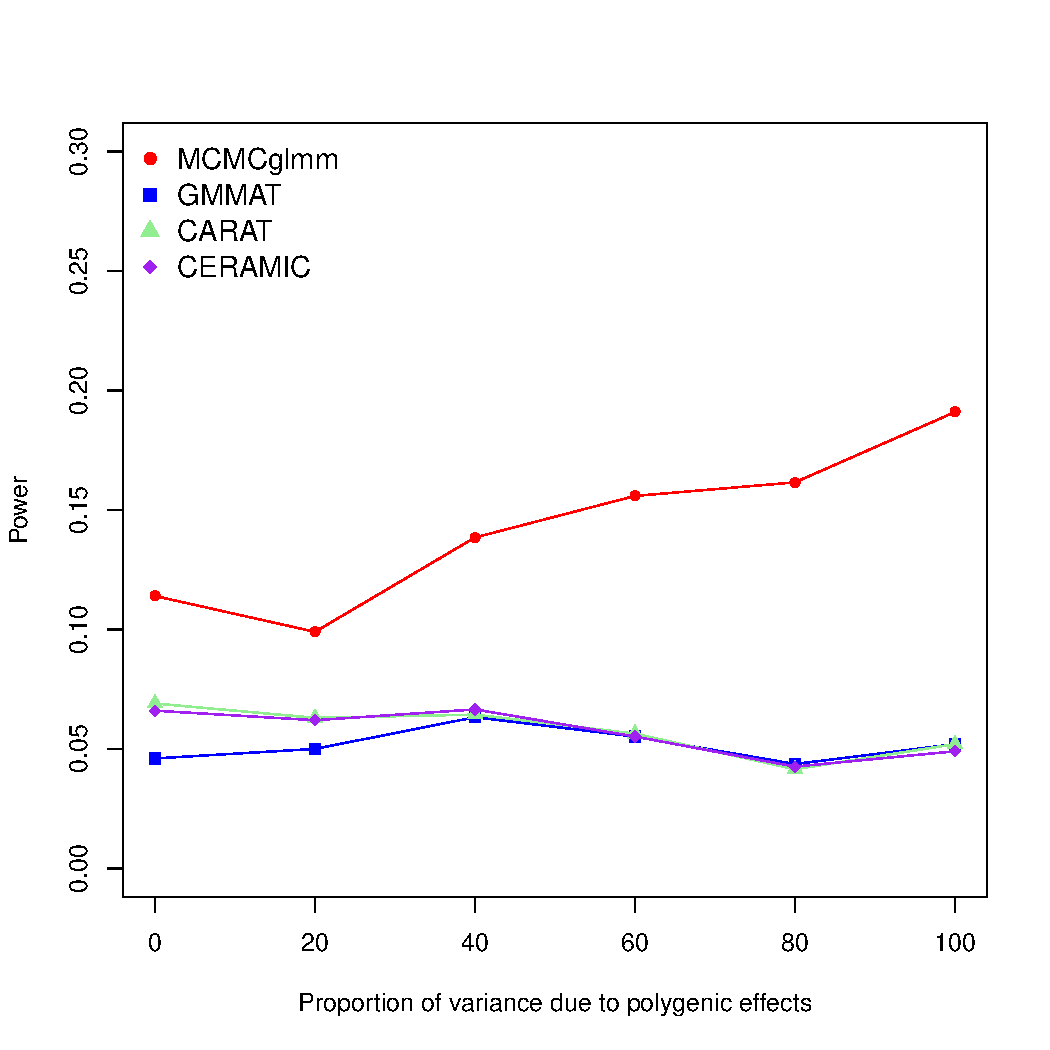
\includegraphics[scale=.45]{power_plot40.pdf}
%\end{center}

\end{document}








